% Author: Dominik Stolte
% Beamer presentation for DSP
% 3.1.2020

\documentclass[aspectratio=32]{beamer}
\usepackage[utf8]{inputenc}
\usepackage[T1]{fontenc} % 256 Zeichen Fonttabelle, statt 128 Zeichen
\usepackage[ngerman]{babel}
\usepackage[scaled]{helvet} 
\usepackage[font=scriptsize]{caption}
\usepackage{bookmark}
\usepackage{booktabs}
\usepackage{verbatim}
\usepackage{graphicx}
\usepackage{textpos}
\usepackage{siunitx}

\title{ELS--Rauscharme Spannungsquellen}
\author{Dominik Stolte, Dennis Henky}
\institute[{Hochschule Mannheim}]{Hochschule Mannheim}
\logo{
\includegraphics[height=0.8cm]{../common/hsma-logo.pdf}\vspace{235pt}}
\date{\today}
\useoutertheme{infolines}

\begin{document} 
\setbeamertemplate{itemize items}[circle]
\setbeamertemplate{navigation symbols}{}

\begin{frame}
  \titlepage{}
\end{frame}

\begin{frame}
  \frametitle{Inhalt}
  \begin{itemize}
    \item Problemstellung
    \item Schaltungssynthese
    \item Auswertung
    \item Fazit
  \end{itemize}
\end{frame}

%------------------------------------------------------------------------------
\section{Problemstellung}
{
  \logo{}
  \setbeamercolor{background canvas}{bg=black!90}
  \setbeamercolor{normal text}{fg=white}
  \setbeamertemplate{footline}{}
  \usebeamercolor*{normal text}
  \begin{frame}
    \centering
    \Large{Problemstellung}
  \end{frame}
}

\begin{frame}
  \frametitle{Problemstellung}
  \centering
  %\includegraphics[width=0.5\textwidth]{bilder/RC-tiefpass.pdf}
  \begin{itemize}
    \item Rauscharme DC Spannungserzeugung
  \end{itemize}
\end{frame}

\begin{frame}
  \frametitle{Rauschen}
  \centering
  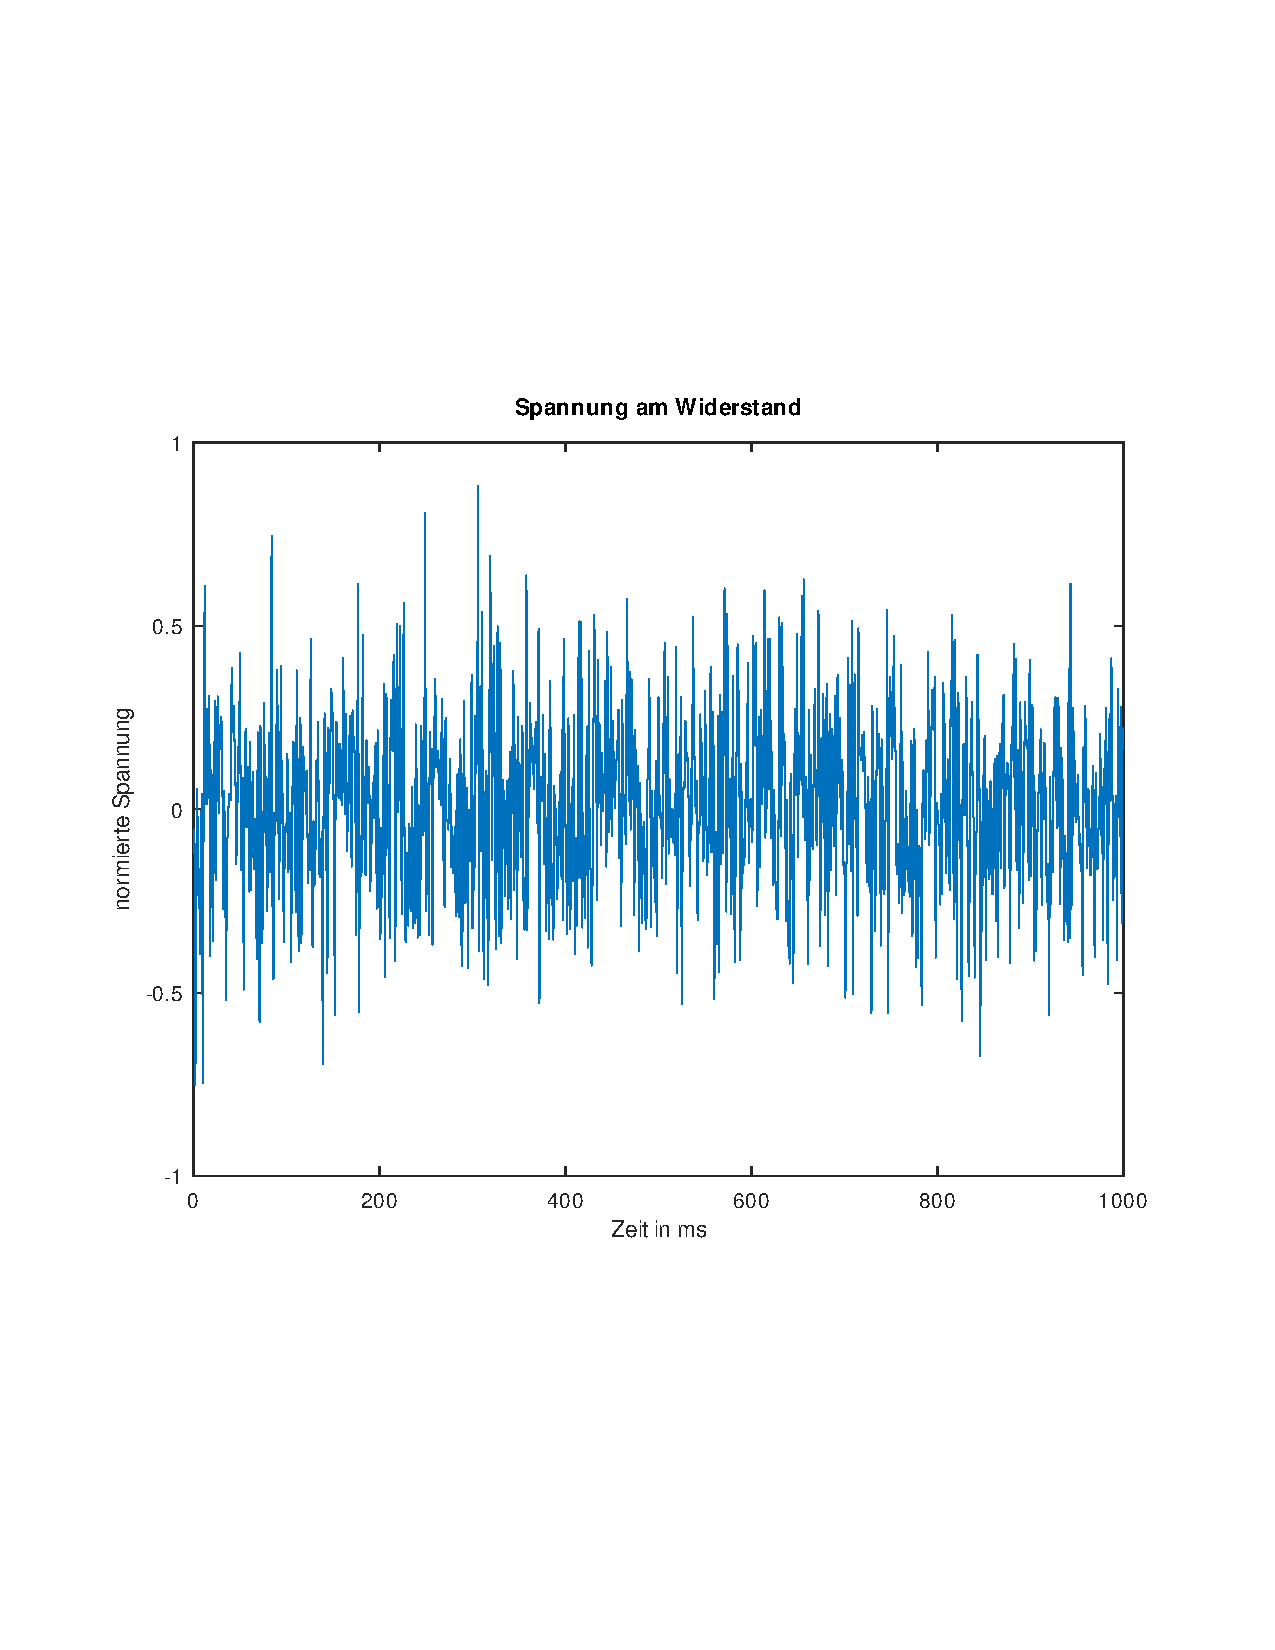
\includegraphics[width=0.5\textwidth]{../common/Simulation/rauschen/spannung.pdf}
  \begin{itemize}
    \item TODO
  \end{itemize}
\end{frame}

\begin{frame}
  \frametitle{Rauschen}
  \centering
  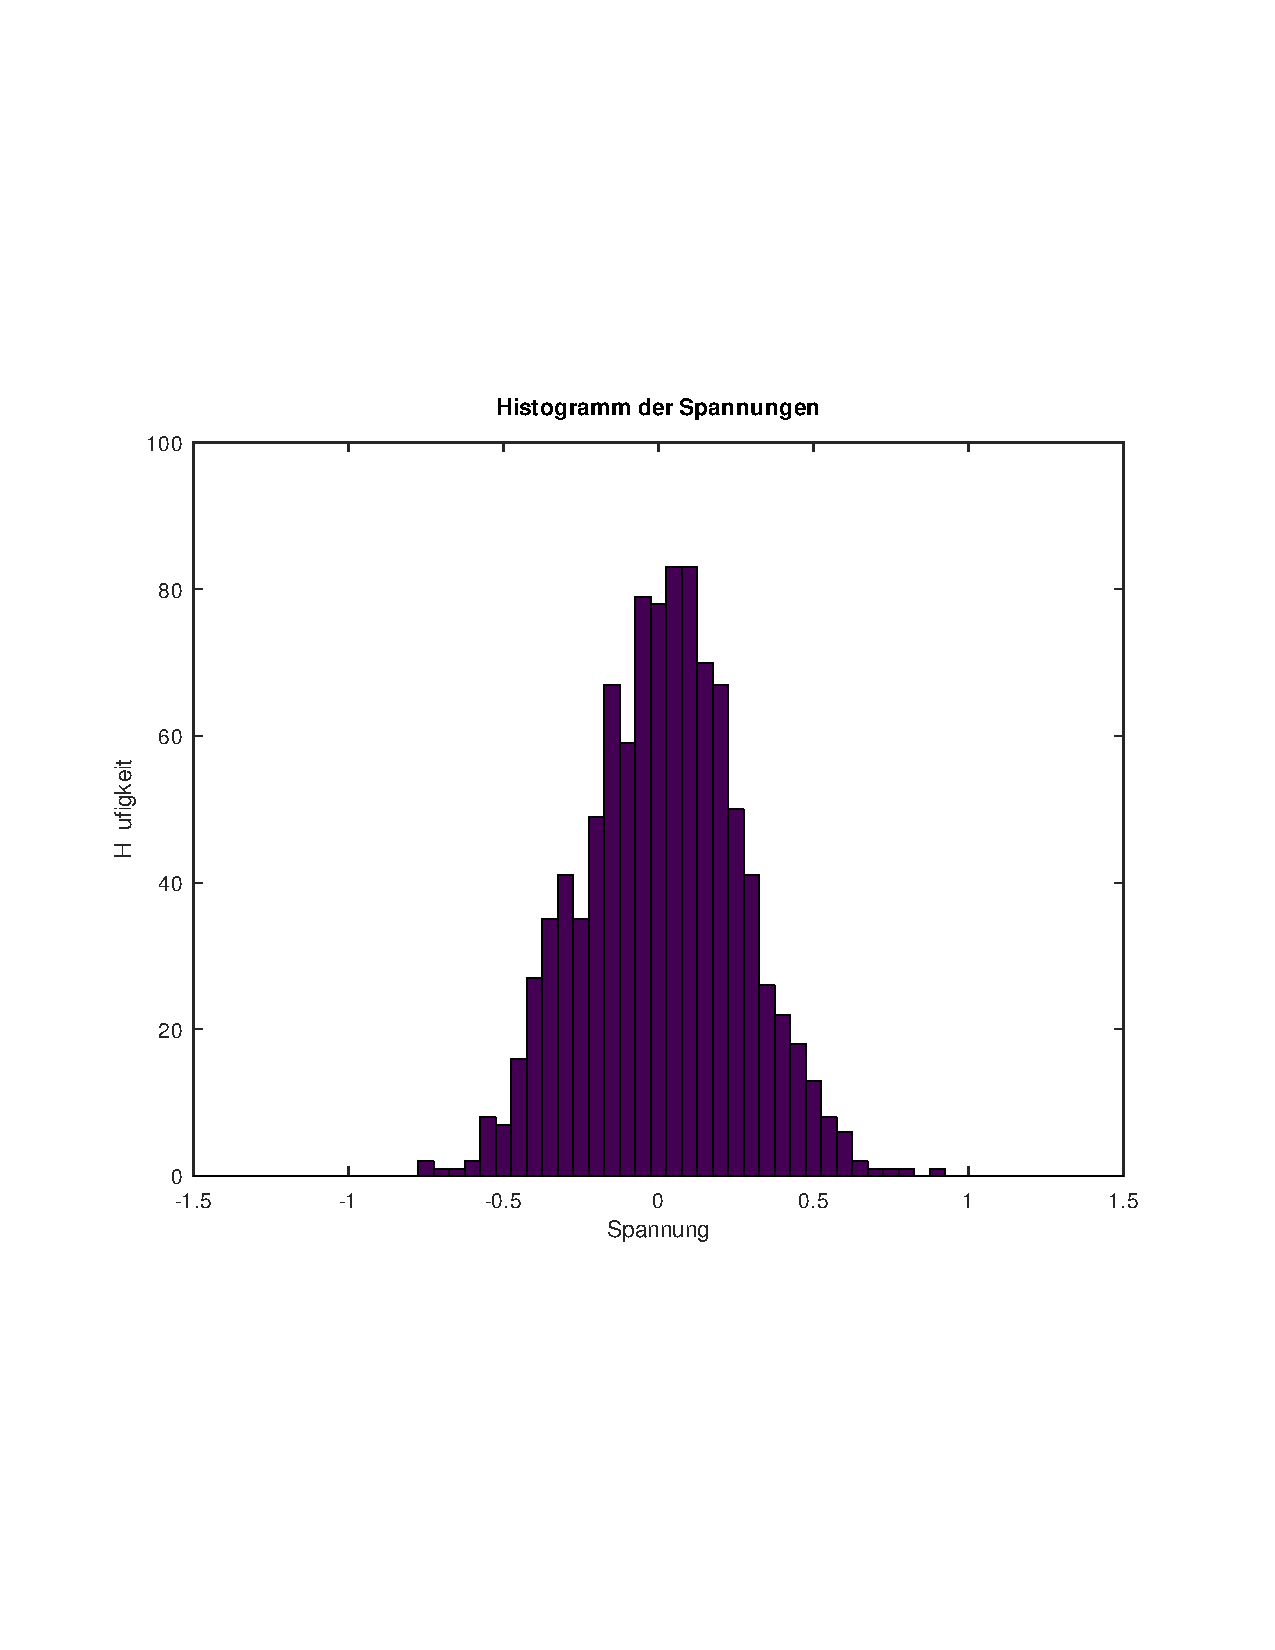
\includegraphics[width=0.5\textwidth]{../common/Simulation/rauschen/haeufigkeit.pdf}
  \begin{itemize}
    \item TODO
  \end{itemize}
\end{frame}

\begin{frame}
  \frametitle{Rauschquellen}
  \centering
  %\includegraphics[width=0.5\textwidth]{bilder/RC-tiefpass.pdf}
  \begin{itemize}
    \item Transistoren 
  \end{itemize}
\end{frame}

\begin{frame}
  \frametitle{Rauchformen}
  \centering
  %\includegraphics[width=0.5\textwidth]{bilder/RC-tiefpass.pdf}
  \begin{itemize}
    \item Transistoren 
  \end{itemize}
\end{frame}

\begin{frame}
  \frametitle{Erzeugung von DC Spannungen aus dem Netz}
  \centering
  %\includegraphics[width=0.5\textwidth]{bilder/RC-tiefpass.pdf}
  \begin{itemize}
    \item Linearregler 
    \begin{itemize}
      \item integriert
      \item Operationsverstärker
      \item diskret
    \end{itemize}
    \item Schaltregler
  \end{itemize}
\end{frame}

%------------------------------------------------------------------------------
\section{Schaltungssynthese}
{
  \logo{}
  \setbeamercolor{background canvas}{bg=black!90}
  \setbeamercolor{normal text}{fg=white}
  \setbeamertemplate{footline}{}
  \usebeamercolor*{normal text}
  \begin{frame}
    \centering
    \Large{Schaltungssynthese}
  \end{frame}
}

\begin{frame}
  \frametitle{Feedbackspannungsteiler}
  \centering
  %\includegraphics[width=0.5\textwidth]{bilder/RC-tiefpass.pdf}
  \begin{itemize}
    \item TODO
  \end{itemize}
\end{frame}

\begin{frame}
  \frametitle{Referenzspannungsquelle}
  \centering
  %\includegraphics[width=0.5\textwidth]{bilder/RC-tiefpass.pdf}
  \begin{itemize}
    \item TODO
  \end{itemize}
\end{frame}

\begin{frame}
  \frametitle{Differentialverstärker}
  \centering
  %\includegraphics[width=0.5\textwidth]{bilder/RC-tiefpass.pdf}
  \begin{itemize}
    \item TODO
  \end{itemize}
\end{frame}

\begin{frame}
  \frametitle{Ausgangsverstärker}
  \centering
  %\includegraphics[width=0.5\textwidth]{bilder/RC-tiefpass.pdf}
  \begin{itemize}
    \item TODO
  \end{itemize}
\end{frame}

%------------------------------------------------------------------------------
\section{Auswertung}
{
  \logo{}
  \setbeamercolor{background canvas}{bg=black!90}
  \setbeamercolor{normal text}{fg=white}
  \setbeamertemplate{footline}{}
  \usebeamercolor*{normal text}
  \begin{frame}
    \centering
    \Large{Auswertung}
  \end{frame}
}

\begin{frame}
  \frametitle{DC Spannungsverlauf}
  \centering
  %\includegraphics[width=0.5\textwidth]{bilder/RC-tiefpass.pdf}
  \begin{itemize}
    \item TODO
  \end{itemize}
\end{frame}

\begin{frame}
  \frametitle{Rauschen}
  \centering
  %\includegraphics[width=0.5\textwidth]{bilder/RC-tiefpass.pdf}
  \begin{itemize}
    \item TODO
  \end{itemize}
\end{frame}


%------------------------------------------------------------------------------
\section{Fazit}
{
  \logo{}
  \setbeamercolor{background canvas}{bg=black!90}
  \setbeamercolor{normal text}{fg=white}
  \setbeamertemplate{footline}{}
  \usebeamercolor*{normal text}
  \begin{frame}
    \centering
    \Large{Fazit}
  \end{frame}
}

\begin{frame}
  \frametitle{Fazit}
  \centering
  %\includegraphics[width=0.5\textwidth]{bilder/RC-tiefpass.pdf}
  \begin{itemize}
    \item Gerede über das Fazit
  \end{itemize}
\end{frame}

\begin{frame}
  \frametitle{Outtakes}
  \centering
  %\includegraphics[width=0.5\textwidth]{bilder/RC-tiefpass.pdf}
  \begin{itemize}
    \item Transistoren 
  \end{itemize}
\end{frame}

\end{document}